\input{../common/header}

\begin{document}

\lecture{ 28 --- Log-Structured File Systems and File Consistency }{\term}{Jeff Zarnett}

\section*{Log-Structured File Systems}
In previous discussions about disk scheduling, we learned that having accesses be random (i.e., non-sequential) is a drag on performance. The key idea behind a log-structured file system is that we could make all writes sequential. For reads, this is not possible, because any data could be requested at any time. But for writes, that's within our control. So let's examine this approach~\cite{OSTEP}.

Both HDD and SSD data storage benefit from this. For the HDD, the idea of writing sequentially minimizes the seek time, which we know from disk scheduling is the thing that is within our control (rotational latency is harder to predict). Extra work is needed at the end to garbage collect the old blocks. We already learned it's not quite as easy as just marking those blocks as unallocated in the OS tracking, but it is not so difficult. The SSD benefits from this because flash memory cannot be overwritten in place; we want to append at the end (even if that's in a random empty block somewhere) and go back and clean up later.

The approach proposed by the inventors of this strategy is explained in their 1992 paper~\cite{log-structured}, which it should be noted predated SSDs in PCs as a standard choice by nearly 20 years. The plan, at a high level, is to write data and metadata into buffers of a given size; when that buffer is full, write it to disk in one sequential write to a big-enough free area. It's just fortunate, in a way, that this strategy works really well for SSDs. That's the nature of research: sometimes an idea doesn't seem that useful until it gets combined with something. 

If we do this sort of writing sequentially, it immediately introduces a question of how will we find things again in the future? The file itself can be moving, after all, as we write more data to it. There must exist some sort of mapping, which is called the \textit{inode map} that is kept up to date. Yes, but finding the map starts to become a problem. The solution is called the \textit{checkpoint region} -- a clearly-noted fixed location on disk that is the location of the pointers to the latest pieces of the inode map and the way to find everything else~\cite{OSTEP}. As you can imagine, this must also contain information on what's free alongside what is allocated.

Writing sequentially, we know, sort of makes no sense in the SSD world because any write location is as good as any other. The main benefit of such a system is that this strategy is already designed for the no-overwrite logic and the TRIM command can be used to indicate what's reached its time to die. 

Writing sequentially is the kind of thing that benefits from a certain economy of scale on HDDs. If you attempted to write just one block at a time, writing sequentially is not that effective, because after writing disk block $A$, if there's a delay, when it's time to write $A+1$ in the next space we will be forced to wait on average for the rotational latency before we can write it. Whereas if we had multiple blocks to go together, we'd write $A, A+1, A+2, A+3...$ in one shot and we'd avoid both seek and rotational latency penalties for 3 of the 4 writes~\cite{OSTEP}. If taken to the limit, if we wrote infinite blocks in a shot we'd amortize the cost of the seek and rotational latency over the infinite write time and it would be negligible.

Okay, infinite write size is not possible and we've identified that a buffer size of 1 block doesn't meet our goals either because the intention is to amortize the cost. Having narrowed it down to somewhere between 1 and infinity is not helpful; we need a goal. And the goal can't be perfection because that's not realistic. Instead, set a target that is a fraction of the theoretical maximum. If we target, let's say, 90\% of the maximum effective rate, that allows setting the buffer size to a specific number. There's nothing magical about 90\% as a target -- but it is reasonable enough. 

Here's the formula for calculating the size of the buffer~\cite{OSTEP}: $D = \dfrac{F}{1-F} \times R_{peak} \times T_{position}$. In this formula, $D$ is the buffer size; $F$ is our target (e.g., 90\% so it'll be 0.9); $R_{peak}$ is the peak disk transfer rate, and $T_{position}$ is the seek and rotational latency cost of moving to the starting point of writing. 

It is clear from the formula that faster disks, both in terms of write speed and positioning time, result in a larger buffer, as does a larger target percentage. There's a temptation to push it to the limit and look for $F$ to be 0.99 or 0.999. And yet, we probably should not do that. 

We introduced a new problem, here. If the system crashes (or loses power) when we have a large buffer that's mostly full, we could lose a lot of progress.  We know that this could happen at any time. LFS addresses this by being prepared for such an eventuality and having a \textit{recovery strategy}. A recovery strategy is exactly what it sounds like, a way to get things back to a consistent state. Let's zoom out for a minute and talk about this in general,  because the idea of a recovery strategy needs a deeper look.

\section*{Consistency Checking and Journalling}

Unfortunately, an error, crash, or power failure or something similar may result in a loss of data or inconsistent data in the file system. The directory structures, pointers, inodes, FCBs, et cetera are all data structures and if they become corrupted it may lead to serious problems.

We could check for inconsistent data periodically (e.g., on system boot up) and many operating systems do so. This is, of course, an operation that will consume a very large amount of time while the whole disk is scanned. The UNIX tool for this is \texttt{fsck} (... not exactly something you want to say out loud) and the Windows tool is \texttt{chkdsk} (check disk). These tools will look for inconsistent states (e.g., a file that claims to be 12 blocks but the linked list contains only 5) and will attempt to repair the data structures. Its level of success depends on the nature of the problem and the implementation of the file system.

Obviously we would like to prevent the problem, if we can. Recall from much earlier the concept of atomic operations: an operation should either succeed completely, or not take place at all. Your first experience with such a structure may have been in version control, when using \texttt{git}: either a commit takes place in its entirety or it is as if it never happened. This approach is used in the Windows NTFS system as well as macOS HFS+ (predecessor to APFS), if journalling is enabled. 

Though we might be familiar, at this point, with the concept of the \textit{transaction}, now let us take a moment to see how it actually works. The simple explanation is: before making any changes, make a list of all the things we plan to do. Then do the things written down. Then we consider the transaction complete. Transactions have \texttt{BEGIN} and \texttt{END} statements, so if a transaction is only partly written down, we will be able to identify that as an incomplete entry in the log file.

All metadata changes are written sequentially to a log file; once the changes are written to the log, control may return to the program that requested the operation. Meanwhile, the log entries are actually carried out. As changes are made, a pointer is updated to indicate which of the log entries have really happened and which have not. When an entire transaction is completed, it is removed from the log file. 

If the system crashes, the log file will contain zero or more transactions. If there are zero there is no problem: nothing was in progress at the time of the crash. If there are some, in progress, it's more interesting. If we have the full transaction information present, we could choose to re-try it and ensure that all changes are applied (or to undo it). Any partial transaction in the log should be aborted: undo any changes that it has done to go back to the beginning. We have to do that because when there is no end-transaction statement, we have no idea what other steps, if any, were supposed to be there. To do that, we walk backwards through the log entries to undo any completed operations and go back to the state before the start of the transaction~\cite{osc}.

Even though a particular write may not have taken place because of a crash, resulting in some data loss, at least the system will always remain in a consistent state. As a side benefit, we can sometimes re-order the writes to get better performance (e.g., schedule them in such a way that we get better disk utilization). 

The approach in Solaris ZFS is similar, but not identical. Blocks are never overwritten with new data. Instead, a transaction writes all data and metadata to new blocks. Only when the transaction is complete, any references to the old blocks are replaced with the location of the new blocks. Then the old pointers and blocks can be cleaned up (reused or disposed of). Because this swap happens at the end and is atomic, we can be sure we'll always be in a good state. If the crash happens before the swap, the old state remains; if the crash happens after, the new one is there.

Before we zoom in on a very specific example of Windows NTFS, one more thing we need to go back for, about log-structured file systems: what is its recovery strategy? Remember that data is written in a segment (a buffer-sized chunk), and when the buffer is full (or after some timeout), it's time to write it to disk. It also uses a log-based system: a checkpoint region has a head-and-tail segment in a sort of linked list, the checkpoint region points to the next segment, and the ``active'' checkpoint region is also periodically updated~\cite{OSTEP}. 

This leaves us with some possibilities about when a crash could occur. If there's nothing out of date when the crash occurs, no problem. The other two possibilities are while writing a segment, and while updating the checkpoint region. 

If the crash happens while writing segment data, that data is probably lost and not coming back. In the simplest case, we could just stop there: recovery is as simple as possible, but the largest amount of data is lost. The alternative is to try to look at what we find in the checkpoint region and try to figure out if any of the updates written in the log were applied to disk; if so, update the file system to reflect what we found, thus getting some of the data and metadata back~\cite{OSTEP}. This is likely only to be partially successful, but it is better than nothing. And this is way faster than scanning the entire disk with \texttt{fsck} or \texttt{chkdsk} because we need only consider things since the last checkpoint region update.

If a crash takes place during updating of the checkpoint region that is a bigger problem. To prevent things from going totally wrong, there are two designated locations for the checkpoint region: start and end of the disk~\cite{OSTEP}. Thus, even in a scenario where the checkpoint region was left in a bad state due to the crash, we can go back to the one recorded earlier, meaning we are never super far away from valid data. 

There is one more option for ensuring data is written to disk without waiting for the buffer to be full or the timeout: the OS may permit something that forces a synchronization of the data to disk. That idea is something that came up in the previous course's interprocess communication topic, when the memory-mapped file topic introduced the \texttt{msync()} system call. Use of that system call blocked further execution until the data was written out, which hurts performance -- but frequently, we don't want to go on until the write is complete. That will come up when we talk about NTFS... 

\subsection*{Example: NTFS (Windows File System)}
Though UNIX and similar systems have often been a focus of the examples, in this case, we will instead examine NTFS, the default file system for Windows since Windows NT and used in 2000, XP, Vista, 7, 8... NTFS supports large disks and large files, and uses journalling. 

NTFS uses several different storage levels~\cite{osi}:

\begin{enumerate}
	\item \textbf{Sector}: Smallest physical storage unit on disk (usually 512 bytes).
	\item \textbf{Cluster}: One or more contiguous sectors (grouped in a power of 2).
	\item \textbf{Volume}: A logical partition on disk, consisting of one or more clusters. 
\end{enumerate}

The cluster is the fundamental unit of allocation of NTFS. This allows the file system to be independent of the size of physical sectors on the disk (which is convenient). A volume contains file system information, a collection of files, and free space. The logical volume may be some of a physical disk, all of one, or spread across multiple physical disks~\cite{osi}. A volume is laid out as follows:

\begin{center}
	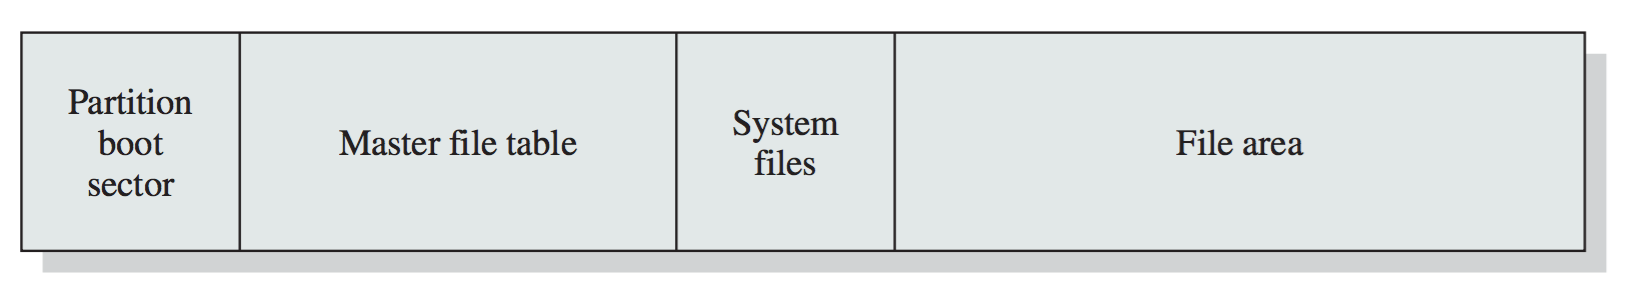
\includegraphics[width=0.6\textwidth]{images/ntfs-volume.png}\\
	Standard layout of an NTFS volume~\cite{osi}.
\end{center}

The Master File Table (MFT) contains information about all the files and folders. Following that, a block is allocated to system files that contain some important system information~\cite{osi}:

\begin{enumerate}
	\item \textbf{MFT2}: Mirror of the first few rows of the MFT (in case the original is damaged).
	\item \textbf{Log File}: The journalling transaction log.
	\item \textbf{Cluster Bitmap}: Bitmap showing which of the clusters are in use.
	\item \textbf{Attribute Definition Table}: Attribute types supported on this volume. (We can ignore this)
\end{enumerate}

NTFS uses journalling to ensure that the file system will be in a consistent state at all times, even after a crash or restart. There is a service responsible for maintaining a log file that will be used to recover in the event that things go wrong.  Note that the goal of recovery is to make sure the system-maintained metadata is in a consistent state; user data can still get lost. This was a decision on the part of Microsoft to make the recovery operations significantly simpler and faster.

Aside: would it be possible to recover user data? The answer is... maybe. 100\% will never be possible because a crash could always happen during writing the logs, so an incomplete transaction will definitely be rolled back. Databases, though, frequently do a better job of retaining the user data. This is not for free, though, because then there must be transaction logs for the data as well. In a database sense, updating the last-login date, for example, is easy to record: change this column on this row from $A$ to $B$. But for a 4K disk block, is this practical? Probably not, because the size of the log would be huge and it would make it more likely that a crash takes place when writing the log rather than writing the disk data. Furthermore, it would also slow down the speed of data writes (have to write the data to the log, then to disk), which we also do not want to do given that the hard drive is already a slow device (as we keep talking about).

The actual implementation of NTFS journalling works as follows~\cite{russ}:

\begin{enumerate}
	\item Record the change(s) in the log file in the cache.
	\item Modify the volume in the cache.
	\item The cache manager flushes the log file to disk.
	\item Only after the log file is flushed to disk, the cache manager flushes the volume changes.
\end{enumerate}

We're sure that this works. Why? Let's enumerate all the possibilities for this:

\begin{itemize}
	\item If the crash happens (1) before step 1, (2) during step 1, (3) between step 1 and 2, (4) during step 2, or (5) between step 2 and 3: nothing was changed on disk, so disk is in a consistent state and there's nothing to do on a restart.
	
	\item If the crash happens during step 3, an incomplete entry is found in the log. Delete it from the log; the volume is in a consistent state.
	
	\item If the crash happens between step 3 and 4, there is an entry in the log that has not been applied. There will be nothing to undo but the system will attempt that anyway. Delete the log entry from the file. The volume is in a consistent state after this.
	
	\item If the crash happens during step 4, the log changes are partially applied. Use the log file to undo them. Delete the log entry from the file. The volume has been restored to a consistent state.
	
	\item If the crash happens after step 4, all changes were already written to disk, so there's nothing to do on a restart.
\end{itemize}

Thus, no matter where in the sequence a crash happens, on system restart, the volume is either in a consistent state or has a clear path to getting to a consistent state.

\section*{Backups}

The journalling recovery approach we've been discussing has to do with putting the file system back into a good state. This means that logical errors can still happen: if you delete the wrong file, it is gone. While it is tempting to say that is the user's error and they can treat this as a ``learning experience'', that's not helpful when that file was important. And besides, deleted-the-wrong-file could happen to anyone (and with AI agents, well, ``you're absolutely right, that was the wrong file to delete and I'm sorry.''\footnote{I don't put emojis in the course notes, but I was tempted to put a skull one here.}). 

Sometimes, we can do ourselves a favour by not cleaning up things immediately! If items are not removed from the log, or old copies of blocks are still available for some period of time, we can maybe go back by undoing or copying the old (retained) blocks over the new ones. Counting on things to just happen to not be deleted yet, though, is wishful and it might work in an extreme data-recovery scenario. Could we formalize this idea into something that's more reliable? Yes, it's called snapshots!

Now that we talked about NTFS, let's restore balance to the universe by talking briefly about APFS -- the newer Apple file system. It uses a copy-on-write mechanism so that changes to metadata never overwrite the old data, which achieves the same goal as journalling without actually going through the two-writes steps where the log is written first and then the changes. 

The snapshot approach allows easily going back to a previous state. Snapshots hang around until they are reclaimed, and reclaiming can be done manually or periodically. Snapshots contain only the metadata, remember. Creating them is easy -- just make a new copy -- but disposing of them will require figuring out what data blocks, if any, can now be deleted for real.

For all of this: none of it helps if something is wrong with the hard drive itself. We often think of them as places for permanent storage of data, but hard drives can and do fail. You know that, if you held my dead 2014 hard drive in your hands. So please, take backups of important data... on different media!

\input{bibliography.tex}
\end{document}